\documentclass[
	a4paper,     		%% Papiergroesse: A4 OBSOLETE
%	twoside,     		%% Zweiseitiges Layout (alternativ: oneside)
	headsepline, 		%% Horizontale Linie unter Kopfzeile
	footsepline, 		%% Horizontale Linie ueber Fusszeile
	titlepage,   		%% Eigenstaendige Titelseite (alternativ: notitlepage)
%	halfparskip, 		%% Halbe Leerzeile zwischen zwei Abschnitten (alternativ: parskip, ...)
	12pt,        		%% Schriftgroesse: 12pt (alternativ: 10pt, 11pt, ...) OBSOLETE
%	bibtotoc,			%% Bibliographie in's Inhaltsverzeichnis aufnehmen
%	liststotoc,			%% Indexe in's Inhaltsverzeichnis aufnehmen
%	smallheadings,		%% Kleine Ueberschriften
%	DIV1,				%% Divisor, Zeilenlänge ca. 70 Zeichen
%	BCOR01cm,			%% Bindekorrektur
%	draft			  	%% Entwurfsmodus, volle/leere Boxen markieren
%	abstracton			%% Titel "`Zusammenfassung"' einschalten
]{scrreprt}

%%%
%%% Pakete
%%%

%%% Glossar
% \usepackage[german]{gloss}
% \newcommand{\acr}[1]{{\small\gloss[word]{#1}}}
% 
% \newcommand{\abk}[1]{#1\xdot}
% \DeclareRobustCommand\xdot{\futurelet\token\Xdot}
% \def\Xdot{\ifx\token\bgroup.\else\ifx\token\egroup.\else
%   \ifx\token\/.\else\ifx\token\ .\else\ifx\token!.\else
%   \ifx\token,.\else\ifx\token:.\else\ifx\token;.\else
%   \ifx\token?.\else\ifx\token/.\else\ifx\token'.\else
%   \ifx\token).\else\ifx\token-.\else\ifx\token+.\else
%   \ifx\token~.\else
%   \ifx\token.\else.\ \fi\fi\fi\fi\fi\fi\fi\fi\fi\fi\fi\fi\fi\fi\fi\fi} 
% \newcommand{\zB}{\mbox{z.\,B}\xdot}

%%% Literaturverzeichnis, deutschen Stil benutzen (dinat)
%%% TODO: funktioniert leider derzeit nicht mit TeXlipse!
%\usepackage[square]{natbib}
%\citestyle{dinat}

%%% Grafik
\usepackage{pstricks}
\usepackage{pst-node}
\usepackage{sudoku}

%%% Subfigures
\usepackage{subfig}

%%% Deutsche Sprache verwenden
\usepackage{ngerman}

%%% Kodierung der Eingabezeichen setzen (fuer dt. Umlaute etc.)
%%% Für Linux: [latin1] für Windows: [ansinew]
\usepackage[utf8]{inputenc}

%%% Zeichen-Kodierung in PDF-Dokumenten
\usepackage[T1]{fontenc}
%\usepackage{ae,aecompl}

%%% Web-Addressen auch mit T1-Encoding
\usepackage[T1]{url}
%%% ... und in tt-Font
\urlstyle{tt}

%%% amsmath, amssymb, amstext: Unterstuetzung div. mathematischer Zeichen etc.
\usepackage{amsmath,amssymb,amstext,units}

%%% pifont: "pifont Xs and Check Marks"
% \usepackage{pifont}

%%% PostScript-Fonts ersetzen
\usepackage{psfrag}

%%% Programmcode einbinden, Listings
\usepackage{listings}

%%% Farb-Unterstuetzung
\usepackage{color}

%%% Tabellen
\usepackage{booktabs}
\usepackage{array}
\usepackage{multirow}
\usepackage{tabularx}
\usepackage{threeparttable}	% Fussnoten in table-Umgebung

%%% Floats strikter positionieren (Option 'H'ere)
\usepackage{float}

%%%
%%% Pakete konfigurieren, Definitionen
%%%

%%% Ueberschriften bis zur Ebene 3 nummerieren
\setcounter{secnumdepth}{3}

\setcounter{tocdepth}{3}

%%% Neue Spaltentypen definieren
\newcolumntype{N}{>{\bfseries\scriptsize}l}
\newcolumntype{V}[1]{
	>{\bfseries\scriptsize\raggedright\hspace{0pt}}p{#1}
}

%%% Ein paar Farbdefinitionen (s. http://texnik.de/listings/listing0.pdf)

\definecolor{hellgelb}{rgb}{1,1,0.8}
\definecolor{hellgrau}{rgb}{0.95,0.95,0.95}
\definecolor{colKeys}{rgb}{0,0,1}
\definecolor{colIdentifier}{rgb}{0,0,0}
\definecolor{colComments}{rgb}{0.7,0.7,0.7}
\definecolor{colString}{rgb}{0,0.5,0}

%%% Konfiguration des listing-Paketes
\lstset{%
	float=hbp,%
	identifierstyle=\color{colIdentifier}, %
 	basicstyle=\ttfamily\small,%
	stringstyle=\ttfamily,%
	keywordstyle=\color{colKeys}, %
	stringstyle=\color{colString}, %
	commentstyle=\color{colComments}, %
	columns=flexible, %
	tabsize=2, %
% 	frame=tb, %
	extendedchars=true, %
	showspaces=false, %
	showstringspaces=false, %
	numbers=left, %
	numberstyle=\tiny, %
	breaklines=true, %
	backgroundcolor=\color{hellgrau}, %
	breakautoindent=true, %
	captionpos=b,%,
	aboveskip=\bigskipamount,%
	belowskip=\medskipamount,%
	escapeinside={(*}{*)}, %
	mathescape=true, %
	language=oz
}

%%% Benoetigte Sprachen laden
% \lstloadlanguages{Pseudo}

%%%
%%% Seitenlayout, Schriften
%%%

%%% scrpage2: KOMA Kopf- und Fusszeile
\usepackage[automark]{scrpage2}

%%% KOMA-Script: Optionen
% \KOMAoptions{fontsize=12pt}
% \KOMAoptions{paper=a4}

%%% EM unterstrichen darstellen
%\usepackage{ulem}

%%% Schrift fuer Captions verkleinern
\setkomafont{captionlabel}{\scriptsize}
\setkomafont{caption}{\usekomafont{captionlabel}}

%%% Schrift fuer Ueberschriften umstellen
%\setkomafont{sectioning}{\normalcolor\bfseries}

%%% Schriften fuer Titel- und Fusszeile umstellen
%\setkomafont{pagehead}{\normalfont\sffamily}
\setkomafont{pagenumber}{\normalfont\rmfamily\slshape}

%%% Unterstuetzung fuer Grafiken
\usepackage[dvips]{graphicx}
\DeclareGraphicsExtensions{.eps}
\graphicspath{{../images}}

%%% Hyperlinks in PS-Dokumenten, Optionen s.o.
\usepackage[%
  dvips,%
  colorlinks=false,%
  breaklinks=true,%
]{hyperref}

\usepackage{breakurl}

%%% Informationen ueber das PDF-Dokument setzen
\hypersetup{
  pdftitle={The Mozart Programming System},%
  pdfauthor={Jan Tammen (jan.tammen@htwg-konstanz.de),%
  			 Tobias Ruf (tobias.ruf@htwg-konstanz.de)},%
  pdfsubject={Wissensbasierte Systeme},%
  pdfcreator={Jan Tammen (jan.tammen@htwg-konstanz.de)},%
  pdfkeywords={Mozart, Oz, multiparadigmisch},
  pdfproducer={\LaTeX\ with package \flqq hyperref\frqq}, %%
%   colorlinks=true,
%  linkcolor=Gray,
%  urlcolor=Gray,
  bookmarksopen=true,
  pdfpagemode=UseOutlines,
  pdfview=FitV, % FitH
  pdfstartview=FitV,
  pdfhighlight=/I,
%   pdfborder=0 0 0, % keine Box um die Links!
  bookmarksnumbered=false,
  plainpages=false,
}

%%% Links im dvips-Mode auch umbrechen
%\usepackage{breakurl}

%%%
%%% Layout der Titelseite
%%%

%%% Titelkopf, erscheint oberhalb des Titels
\titlehead{
	\begin{figure}[H]
		\centering
		
\includegraphics[width=\textwidth]{../images/htwg-logo}
	\end{figure}
}

%%%% Subject, erscheint oberhalb des Titels
\subject{Wissensbasierte Systeme, SS 07}

%%% Titel
\title{The Mozart Programming System}


%%% Publisher, hier: Verantwortlicher Prof.
\publishers{%
	\small
  Prof.\ Dr.\,Hedtstück, HTWG Konstanz
}

%%%% Autor. Weitere Autoren mit \and{<Name>} hinzufuegen
\author{%
	Tobias Ruf
	\and{%
		Jan Tammen
	}%
}%

%%% Datum setzen
\date{\today}

%%% Rueckseite der Titelseite
\lowertitleback{%
	\footnotesize%
	Erstellt mit \LaTeXe\ unter Verwendung des \KOMAScript-Pakets.
}

%%%
%%% Header und Footer
%%%

\pagestyle{scrheadings}

%%% Kopfzeile in den Rand ragen lassen
%\setheadwidth{textwithmarginpar}

%%% Fusszeile in den Rand ragen lassen
%\setfootwidth{head}

%%% \automark[rechte Seite]{linke Seite}
%\automark[subsection]{section}

%% Header links -- section
%\ihead[]{\rightmark}

%% Header rechts -- chapter
%\ohead[]{\leftmark}

%% Header mittig -- leer
\chead[]{}

%% Footer mittig -- leer
\cfoot[]{}

%% Footer rechts -- Seitenzahl
\ofoot[]{\thepage}

%%% Footer links -- Titel der Arbeit
\ifoot[]{\footnotesize{The Mozart Programming System}}

%%%
%%% Sonstiges
%%%

%%% Glossar und Index erstellen 
% \makegloss
% \makeindex

%%%
%%% Beginn Hauptdokument
%%%
\begin{document}

%%% Titelseite erstellen
\maketitle

%%% Inhaltsverzeichnis erstellen
%\newpage
\tableofcontents

%%% Bildverzeichnis erstellen
%\newpage
%\listoffigures

%%% Tabellenverzeichnis erstellen
%\newpage
%\listoftables

%%%
%%% Beginn Inhalt
%%%
\chapter{Einleitung}
\begin{frame}{Mozart - Einleitung}
  \begin{itemize}
    \item Mozart implementiert die multiparadigmische Programmiersprache Oz
    \item Forschungsprojekt seit ca.\ 1995 (B, D, S)
    \item Oz ist plattformunabhängig (Byte-Code ähnlich wie Java)
    \item Open-Source-Lizenz
  \end{itemize}
\end{frame}

\begin{frame}{Mozart - Features}
  \begin{itemize}
    \item Unterstützung mehrerer Programmierparadigmen
    \item Nebenläufigkeit (Threads, Synchronisation)
    \item Transparente Verteilung
    \item Dynamische Typisierung
  \end{itemize}
\end{frame}

\begin{frame}{Oz - Programmiermodell (OPM)}
  \begin{itemize}
    \item Berechnungen laufen in sog.\ "`Spaces"' (Berechnungsraum) ab
    \item \textsl{Aktoren} kommunizieren darin über einen gemeinsamen 
    \textsl{Speicher}, können Information ablegen und abrufen
    \item Grundlage von Oz: Concurrent Constraint Programming, Erweiterungen 
    durch \textsl{syntactic sugar}
  \end{itemize}
\end{frame}

\begin{frame}{Oz - Datentypen}
  \begin{itemize}
    \item Basisdatentypen: \texttt{Number: Int, Float, Char}
    \item Zusammengesetzte Typen: \texttt{Record: Tuple, Literal, Bool}
    \item \texttt{Chunk}: erlaubt Erstellung abstrakter Datentypen, vordefiniert
    z.\,B.\ \texttt{Array, Dictionary, Class}
    \item \texttt{Thread, Space, ByteString, \ldots}
  \end{itemize}
\end{frame}

\chapter{Paradigmen} \label{chapter:paradigmen}
\subsection{Concurrent Constraint Programming}
\begin{frame}{Constraint Programming}
  \begin{itemize}
    \item Constraint: logische Formel, welche den möglichen Wertebereich von 
    Variablen einschränkt (engl.\ to constrain)
    \item Elementarer Constraint: z.\,B.\: $X=Y \quad X=23 \quad 
    X=\mathrm{pair}(Y\,Z)$
    \item \textsl{finite domain} Constraint: $X::1\#42$, Beschränkung von $X$ 
    auf ganze Zahlen zwischen 1 und 42
  \end{itemize}
\end{frame}

\begin{frame}{Constraint Programming: finite domain problems}
  \begin{itemize}
    \item Lösung kombinatorischer Probleme, z.\,B.\ "`N Damen"'-, 
    "`Graphfärbe"'-Problem mithilfe von \textsl{Constraint Propagation}
    \item Hier: Speicher $\equiv$ \textsl{Constraint Store}, Aktoren $\equiv$ 
    \textsl{Propagators}
    \item Constraint Store speichert Konjunktion aus elementaren Constraints, 
    z.\,B.\ $X \in 0\#5 \wedge Y = 8 \wedge Z \in 13\#23$
    \item Propagators führen komplexte Constraints ein, z.\,B.\ $X < Y$ oder 
    $X^2 + Y^2 = Z^2$
  \end{itemize}
\end{frame}

\begin{frame}{Constraint Programming: Beispiel Propagation}
  \begin{itemize}
    \item Constraint Store enthält: $X \in 0\#9 \wedge Y \in 0\#9$
    \item Propagator 1 ($P_1$): $X + Y = 9$, Propagator 2 ($P_2$): $2 \cdot X + 
    4 \cdot Y = 24$
  \end{itemize}
  \pause
  \begin{enumerate}[<+->]
    \item $P_2$ schränkt ein: $X \in 0\#8 \quad Y \in 2\#6$
    \item $P_1$ schränkt ein: $X \in 3\#7 \quad Y \in 2\#6$
    \item \ldots
    \item $P_2$ stellt fest: $X = 6 \quad Y = 3$
  \end{enumerate}
\end{frame}

\begin{frame}{Constraint Programming: Distribuierung}
  \begin{itemize}
    \item Constraint Propagation ist keine vollständige Lösungsmethode
    \item Abhilfe: "`Distribution"'
    \item Unterteilung des Suchraums in mehrere Spaces (mithilfe eines
    Suchbaums) 
    \item Dazu: "`Erfinden"' eines neuen Constraints für den linken Teilbaum;
    dessen Negation für den rechten Teilbaum
  \end{itemize}
\end{frame}

\begin{frame}{Constraint Programming in Oz: "`Send More Money"'}
  \begin{block}{Das "`Send More Money"'-Problem}
    \begin{description}
      \item[Gegeben] $SEND + MORE = MONEY$
      \item[Gesucht] Ziffern (0-9) für die Buchstaben
      \item[Bedingungen] Ziffern paarweise verschieden, $S \neq 0, M \neq 0$
      \item[Lösung] $9567 + 1085 = 10652$
    \end{description}
  \end{block}
\end{frame}

\begin{frame}{Constraint Programming in Oz}
  \lstinputlisting[firstline=2]{../oz-constraint.oz}
  \href{run:oz-constraint.oz}{\beamergotobutton{OPI starten}} 
\end{frame}

\subsection{Funktionale Programmierung}
\begin{frame}{Funktionale Programmierung}
  \begin{itemize}
    \item Grundidee: Auswertung (mathematischer) Ausdrücke
    \item Ziel: Programmverifikation vereinfachen (s.\ $\lambda$-Kalkül)
    \item Gewöhnungsbedürftig: Keine Schleifen und Zuweisungen, sondern 
    Rekursion!
  \end{itemize}
\end{frame}

\begin{frame}{Funktionale Programmierung in Oz}
  \lstinputlisting{../oz-funktional2.oz}
  \href{run:oz-funktional2.oz}{\beamergotobutton{OPI starten}} 
\end{frame}

\subsection{Objektorientierte Programmierung}
\begin{frame}{Klassen und Objekte}
  \begin{itemize}
    \item Klasse: Datenstruktur mit Methodentabelle und Attributnamen
    \item Objekt: Datenstruktur mit Komponenten, darunter u.\,a.\:
	  \begin{itemize}
        \item Klasse
        \item Zustand
      \end{itemize}
        \item Besonderheiten: Unterstützung für Mehrfachvererbung, sog.\ 
        "`Features"'
  \end{itemize}
\end{frame}

\begin{frame}{Objektorientierte Programmierung in Oz}
  \lstinputlisting{../oz-oop.oz}
  \href{run:oz-oop.oz}{\beamergotobutton{OPI starten}} 
\end{frame}

\subsection{Logische Programmierung}
\begin{frame}{Logische Programmierung}
  \begin{itemize}
    \item Grundidee: Berechnung als \textsl{Deduktion}
    \item Jedem bekannt: PROLOG
    \item Aus der Idee der logischen Programmierung ging 
    Constraintprogrammierung hervor
  \end{itemize}
\end{frame}

\begin{frame}{Logische Programmierung in Oz}
  \lstinputlisting{../oz-logisch.oz}
  \href{run:oz-logisch.oz}{\beamergotobutton{OPI starten}} 
\end{frame}

\chapter{System Module}
%\subsection{Überblick}
\begin{frame}{System Module - Überblick} 
  \begin{itemize}
    \item Erweiterung der Oz Base Environment
    \item Ermöglichen effektiveres und effizienteres Entwickeln
    \item Module für verschiedene Einsatzgebiete
    \item Sozusagen die Standardbibliothek von Oz
  \end{itemize}
\end{frame}
 
\subsection{Application Programming} 
\begin{frame}{Application Programming}
  \begin{itemize} 
    \item 2 Module für Applikationen und das Laden von Modulen
    \item Module
    \begin{description}
      \item[\texttt{Application}] Zugriff auf die Argumente einer
      Applikation
      \begin{itemize} 
  	    \item Vergleichbar mit \texttt{String args[]} in Java
  	    \item Parsen der übergebenen Argumente
	  \end{itemize}
      \item[\texttt{Module}]Laden von Modulen
    \end{description}
  \end{itemize}
\end{frame}
 
\subsection{Constraint Programming}
\begin{frame}{Constraint Programming}
  \begin{itemize}
    \item Erweiterungen für Constraint Programming
    \item Insgesamt 7 Module, die Semantik und Syntax erweitern
    \item Module
    \begin{description}
      \item[\texttt{Search}] Unterstützung von verschiedenen Suchmaschinen
      \item[\texttt{FD}] Erweiterungen für finite domain Constraints
      \item[\texttt{Schedule}] Unterstützung für Scheduling-Anwendungen
      \item[\texttt{FS}] Erweiterung von finite Domain Constraints auf Mengen
      \item[\texttt{RecordC}] Records als Constraints
      \item[\texttt{Combinator}] Kombinatoren für Constraints, z.B. \texttt{or}
      \item[\texttt{Space}] Erweiterung für die Spaces
    \end{description}
  \end{itemize}
\end{frame}

\begin{frame}{Modul \texttt{Search}}
  \begin{itemize}
    \item \textbf{Basis Suchmaschinen} - Suche nach einer Lösung, allen Lösungen oder
    den besten Lösungen.
    \item \textbf{Universelle Suchmaschinen} - Parameterisierte Suche
    \begin{itemize}
      \item Recomputation - Reduzierung des Suchraums (Space)
      \item Beenden der Suche
      \item Verschiedene Ausgabe-Modi
    \end{itemize}
    \item \textbf{Parallele Suche} - Verteilung der Suche auf Rechnern im Netzwerk
    \begin{itemize}
      \item Verteilung durch Aufteilung des Suchbaum in Untersuchbäume
      \item Nur von Vorteil, wenn Suchbaum groß genug und gut unterteilbar
    \end{itemize}
  \end{itemize}
\end{frame}

\begin{frame}{Finite Domain Constraints: \texttt{FD} }
  \begin{itemize}
    \item Erweiterung des Telling auf den Constraint Store für
     Datenstrukturen
    \item Reflection für Domains
    \item Verschiedene vordefinierte Propagatoren, z.B. Generic Propagators
    oder 0/1 Propagators (binär) 
  \end{itemize}
\end{frame}

\begin{frame}{Scheduling Unterstützung: \texttt{Schedule}}
    \begin{itemize}
      \item Propagatoren und Verteiler für Scheduling-Anwendungen
      \item \textit{Serialization for unary resources} - Anordnung von Tasks, die
      gleiche Ressource benötigen, ohne zeitliche Überlappung
      \item Verteilung der Tasks, so dass jede benötigte Ressource \textit{serialized}
      ist
      \item Kumulatives Scheduling - Kapazität einer Ressource darf nicht
      überschritten werden
    \end{itemize} 
\end{frame}

\begin{frame}{Finite Set Constraints: \texttt{FS}}
  \begin{itemize}
    \item Neue Constraint-Art
    \item Assoziation einer $n$-elementigen Menge mit $n$ finite Domain
      Variablen
    \item Mengen von Constraint Variablen sehr nützlich bei kombinatorischer
      Problemlösung und Natural Language Processing
    \item Prozeduren, Propagator usw. für den Umgang mit Finite Set Constraints 
  \end{itemize}
\end{frame}

\begin{frame}{First-class Computation Spaces: \texttt{Space}}
  \begin{itemize}
    \item Zur Programmierung von Interferenzmaschinen 
    \item Prozeduren um mit Computation Spaces umzugehen
  \end{itemize} 
\end{frame}



\subsection{Verteilte Programmierung}
\begin{frame}{Verteilte Programmierung}
  \begin{itemize}
    \item Zur Entwicklung von verteilten Anwendungen
    \item Module
    \begin{description}
      \item[\texttt{Connection}] Ticket-basierter Verbindungsaufbau zwischen unabhängigen Oz
      Prozessen, auch lokal. Ticket ist ein String, der übertragen wird.
      \begin{itemize}
        \item One-to-one - Einzelverbindungen
        \item Many-to-one - Mehrere Verbindungen mit gleichem Ticket
      \end{itemize}
      \item[\texttt{Remote}] Remotesteuerung anderer Oz Prozesse über das
      Netzwerk. 
      \item[\texttt{URL}] Erzeugen und Manipulieren von URLs, für das WWW und
      Dateisystem
    \end{description}
  \end{itemize}
\end{frame} 

\begin{frame}{Verteilte Programmierung}
  \begin{itemize}
    \item Weitere Module:
    \begin{description}
      \item[\texttt{Resolve}] Auflösen von URLs zur einfacheren Auffindung von Daten
      \item[\texttt{Fault}] Erkennung und Behandlung von Fehlern in der Verteilung
      \item[\texttt{Discovery}] Lokation von Diensten (Oz-Server) im Netzwerk
      \item[\texttt{DPInint}] Initialisierung und Konfiguration der Verteilungsschicht
      \item[\texttt{DPStatistics}] Abfrage von statistischen Informationen
    \end{description}
  \end{itemize}
\end{frame}

\subsection{Open Programming}
\begin{frame}{Open Programming}
  \begin{itemize}
    \item Verbindung zum Rest der \textit{computational world}
    \item Module
    \begin{description}
      \item[\texttt{Open}] Zugriff auf Dateien, Sockets und Pipes 
      \item[\texttt{OS}] Support für Betriebssysteme. Prozeduren zur
      Interaktion mit dem Betriebssystem, z.B. Exceptions falls Fehler auftretten
    \end{description}
  \end{itemize}
\end{frame}

\subsection{System Programmierung}
\begin{frame}{System Programmierung}
  \begin{itemize}
    \item Weitere Funktionalität für die Mozart Engine
    \item Module
    \begin{description}
      \item[\texttt{Pickle}] Persistente Speicherung von zustandlosen Werten
      \item[\texttt{Property}] Operationen auf Eigenschaften (Properties)
      \item[\texttt{Error}] Formatierung von Fehlermeldungen, z.B. Exceptions
      \item[\texttt{ErrorFormatters}] Vordefinierte Fehlerformatierungen, z.B.
      \texttt{os} Fehler des Betriebssystems
      \item[\texttt{Finalize}] Automatische Freigabe von Resourcen, bei
      gekapselten Daten
      \item[\texttt{System}] Prozeduren für die Mozart Engine, z.B. Drucken
    \end{description} 
  \end{itemize}
\end{frame}

\subsection{Window Programming}
\begin{frame}{Window Programming}
  \begin{itemize}
    \item Programmierung von Benutzeroberflächen mit Tk
    \item Module
    \begin{description}
      \item[\texttt{Tk}] Modul zur GUI Programmierung. Verschiedene Klassen für
      die Kommunikation zwischen der Graphic Engine und der Mozart Engine
      \item[\texttt{TkTools}] Graphische Tools, vordefinierte Klassen für
      Dialoge, Menüs usw. 
    \end{description}
  \end{itemize}
\end{frame}

\chapter{Projekte und aktuelle Entwicklungen}
Schließlich noch 2 kurze Beispiele was in Form von Projekten rund um Mozart und
Oz passiert. Zunächst wird ein sehr interessantes Projekt, \textsl{Strasheela},
vorgestellt, das sich mit dem regelbasierten Komponieren von Musik beschäftigt.
Außerdem wird kurz auf einen Versuch eingegangen, bei dem Mozart und Oz in die
Eclipse IDE integriert werden soll. 

\section{Strasheela}

Das von Torsten Anders veröffentliche
\textsl{Strasheela}\footnote{\url{http://strasheela.sourceforge.net/strasheela/doc/}} 
stellt ein in Mozart/Oz implementiertes System dar, mit dem Constraintbasiert
Musik erzeugt werden kann. Der Benutzer gibt deklarativ, in Form von Oz-Code, eine
Musiktheorie an. Oz versucht durch Suche die definierten Constraints zu
terminieren. Um diese Lösungen auch als Musik zu hören, bietet Strasheela die
Möglichkeit die Lösung als MIDI-Datei zu exportieren.

Ein Beispiel, das Strasheela mitliefert, ist sind die so genannten 
\textsl{All-Interval Series}. Diese Musiktheorie stammt aus dem Feld der 
seriellen Musik (serial Musik), siehe \cite{url:serielleMusik}. Eine Serie von 
Tönen besteht in diesem Beispiel aus 12 Tönen einer Tonleiter, die für jede 
Serie nur einmal verwendet werden dürfen. Außerdem müssen die Abstände zwischen 
den einzelnen Tönen eindeutig sein, d.h. pro Serie darf jeder Abstand 
(Intervall) nur einmal vorkommen. Laut \cite{url:strasheela} gibt es für dieses 
Problem 3856 Lösungen, die von Mozart alle gefunden werden, siehe Abbildung 
\ref{fig:strasheela-search}.

\begin{figure}
 \centering
 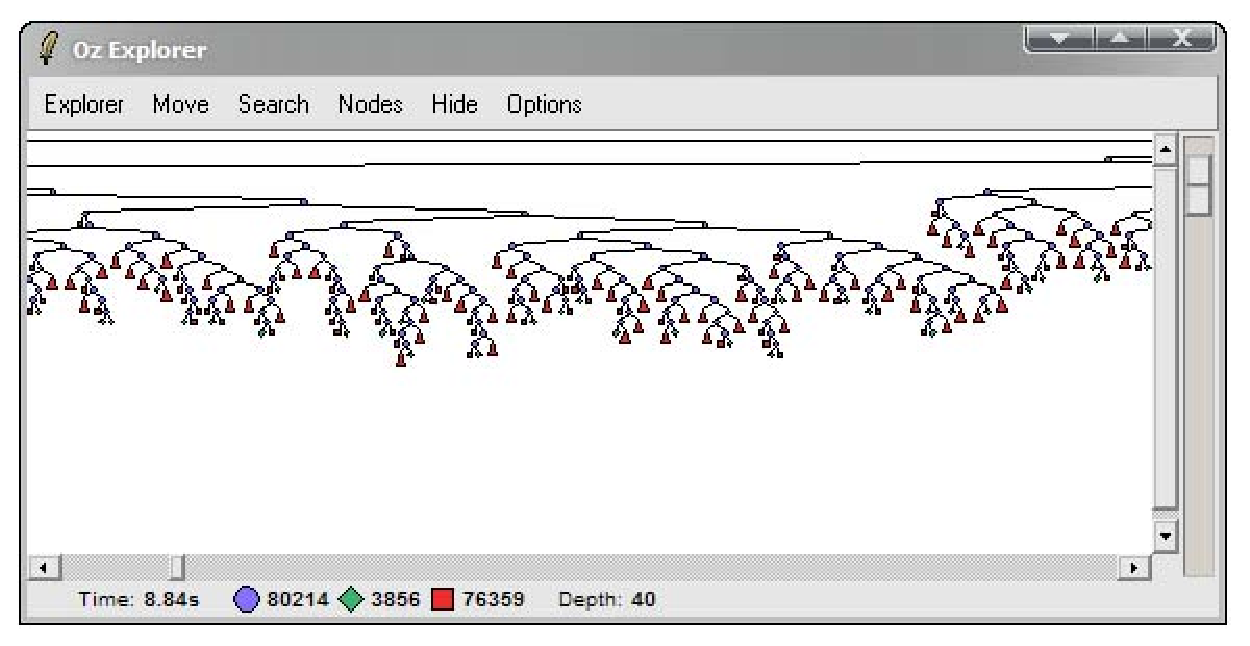
\includegraphics[width=0.6\textwidth]{../images/strasheela-search}
 \caption{Suche nach allen Lösungen von \textsl{All-Interval Series}, grüne
 Raute}
 \label{fig:strasheela-search}
\end{figure}


\section{MozEclipse}

Im Februar diesen Jahres startete Craig Ugoretz das Projekt 
\textsl{MozEclipse}\footnote{\url{http://gforge.info.ucl.ac.be/projects/mozeclipse/}}. 
Ziel dieses Projekts ist es, Mozart und Oz in die Eclipse IDE zu integrieren. 
Durch die Integration soll der Bekanntheitsgrad von Mozart/Oz steigen. Momentan 
ist Mozart in den Emacs integriert, der vor allem Anfängern einige 
Schwierigkeiten bereitet. Durch die Integration in Eclipse sollen die Hemmungen 
beseitigt werden, da viele Anwender gut mit Eclipse vertraut sind. Leider ist 
die Zukunft dieses Projekts noch sehr ungewiss, da es seit dem Anlegen der 
Projekt-Homepage keine weiteren Aktivitäten gab.

%%%
%%% Anhaenge: Glossar, Bibliographie...
%%%

%\cleardoublepage % oder \clearpage
%\phantomsection 

\appendix
\pdfbookmark[-1]{\appendixname}{\appendixname} 

\chapter{Quellcode Sudoku-Löser (GUI)}
\lstinputlisting[label={lst:sudoku-solver-gui}, caption={Graphische Ausgabe der
Sudoku-Lösung}, firstline=66, mathescape=false]{../sudokuSolver.oz}

%%% Bibliographie-Stil
% abbrvdin, alphadin, plaindin, unsrtdin
\bibliographystyle{alphadin}

%%% Anstatt 'Literatur' -> 'Quellen'
\renewcommand{\bibname}{Quellen}

%%% Bibliographie ausgeben
\bibliography{Literatur}

%%% Glossar ausgeben
%\printgloss{Glossar}

\end{document}
